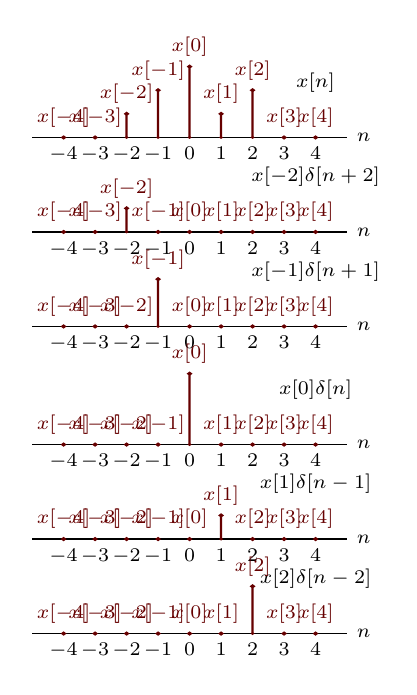
\begin{tikzpicture}[xscale=0.4, yscale=0.3, every label/.append style={text=black}]

	\def\nmin{-4}
	\def\nmax{4}	
	
		
	\begin{scope}	
		\def\x{{0, 0, 1, 2, 3, 1, 2, 0, 0}}		
		\draw (\nmin-1, 0) -- (\nmax+1,0) node[anchor=west] {\scriptsize $n$};
		\foreach \n in {\nmin, ..., \nmax}
		{
			\node at (\n, 0) [anchor=north] {\scriptsize $\n$};
		}
		\node at (\nmax,1.5) [anchor=south] {\scriptsize $x[n]$};
		
		\foreach \n/\a in {0/{-4},1/{-3}, 2/{-2}, 3/{-1}, 4/{0}, 5/{1}, 6/{2}, 7/{3}, 8/{4}}
		{
			\pgfmathparse{\x[\n]}
			\edef\xn{\pgfmathresult}	
			\ifthenelse{\xn > 0}
			{

				\draw[red!40!black, thick, fill=red!40!black]  (\n + \nmin, 0) -- ++(0, \xn) circle (1pt) node[anchor=south] {\scriptsize $x[\a]$};
			}
			{
				\draw[red!40!black, fill=red!40!black] (\n+ \nmin,  0) circle (1pt);
			}
		}
	\end{scope}	
	
	\pause
	
	\begin{scope}[yshift=-4cm]
		\def\x{{0, 0, 1, 0, 0, 0, 0, 0, 0}}		
		\draw (\nmin-1, 0) -- (\nmax+1,0) node[anchor=west] {\scriptsize $n$};
		\foreach \n in {\nmin, ..., \nmax}
		{
			\node at (\n, 0) [anchor=north] {\scriptsize $\n$};
		}
		\node at (\nmax,1.5) [anchor=south] {\scriptsize $x[-2]\delta[n+2]$};
		
		\foreach \n/\a in {0/{-4},1/{-3}, 2/{-2}, 3/{-1}, 4/{0}, 5/{1}, 6/{2}, 7/{3}, 8/{4}}
		{
			\pgfmathparse{\x[\n]}
			\edef\xn{\pgfmathresult}	
			\ifthenelse{\xn > 0}
			{

				\draw[red!40!black, thick, fill=red!40!black]  (\n + \nmin, 0) -- ++(0, \xn) circle (1pt) node[anchor=south] {\scriptsize $x[\a]$};
			}
			{
				\draw[red!40!black, fill=red!40!black] (\n+ \nmin,  0) circle (1pt);
			}
		}
	\end{scope}		

	\pause

	\begin{scope}[yshift=-8cm]
		\def\x{{0, 0, 0, 2, 0, 0, 0, 0, 0}}		
		\draw (\nmin-1, 0) -- (\nmax+1,0) node[anchor=west] {\scriptsize $n$};
		\foreach \n in {\nmin, ..., \nmax}
		{
			\node at (\n, 0) [anchor=north] {\scriptsize $\n$};
		}
		\node at (\nmax,1.5) [anchor=south] {\scriptsize $x[-1]\delta[n+1]$};
		
		\foreach \n/\a in {0/{-4},1/{-3}, 2/{-2}, 3/{-1}, 4/{0}, 5/{1}, 6/{2}, 7/{3}, 8/{4}}
		{
			\pgfmathparse{\x[\n]}
			\edef\xn{\pgfmathresult}	
			\ifthenelse{\xn > 0}
			{

				\draw[red!40!black, thick, fill=red!40!black]  (\n + \nmin, 0) -- ++(0, \xn) circle (1pt) node[anchor=south] {\scriptsize $x[\a]$};
			}
			{
				\draw[red!40!black, fill=red!40!black] (\n+ \nmin,  0) circle (1pt);
			}
		}
	\end{scope}		
	
	\pause	
%	
	\begin{scope}[yshift=-13cm]
		\def\x{{0, 0, 0, 0, 3, 0, 0, 0, 0}}		
		\draw (\nmin-1, 0) -- (\nmax+1,0) node[anchor=west] {\scriptsize $n$};
		\foreach \n in {\nmin, ..., \nmax}
		{
			\node at (\n, 0) [anchor=north] {\scriptsize $\n$};
		}
		\node at (\nmax,1.5) [anchor=south] {\scriptsize $x[0]\delta[n]$};
		
		\foreach \n/\a in {0/{-4},1/{-3}, 2/{-2}, 3/{-1}, 4/{0}, 5/{1}, 6/{2}, 7/{3}, 8/{4}}
		{
			\pgfmathparse{\x[\n]}
			\edef\xn{\pgfmathresult}	
			\ifthenelse{\xn > 0}
			{

				\draw[red!40!black, thick, fill=red!40!black]  (\n + \nmin, 0) -- ++(0, \xn) circle (1pt) node[anchor=south] {\scriptsize $x[\a]$};
			}
			{
				\draw[red!40!black, fill=red!40!black] (\n+ \nmin,  0) circle (1pt);
			}
		}
	\end{scope}		
	
	\pause	
	
	\begin{scope}[yshift=-17cm]
		\def\x{{0, 0, 0, 0, 0, 1, 0, 0, 0}}		
		\draw (\nmin-1, 0) -- (\nmax+1,0) node[anchor=west] {\scriptsize $n$};
		\foreach \n in {\nmin, ..., \nmax}
		{
			\node at (\n, 0) [anchor=north] {\scriptsize $\n$};
		}
		\node at (\nmax,1.5) [anchor=south] {\scriptsize $x[1]\delta[n-1]$};
		
		\foreach \n/\a in {0/{-4},1/{-3}, 2/{-2}, 3/{-1}, 4/{0}, 5/{1}, 6/{2}, 7/{3}, 8/{4}}
		{
			\pgfmathparse{\x[\n]}
			\edef\xn{\pgfmathresult}	
			\ifthenelse{\xn > 0}
			{

				\draw[red!40!black, thick, fill=red!40!black]  (\n + \nmin, 0) -- ++(0, \xn) circle (1pt) node[anchor=south] {\scriptsize $x[\a]$};
			}
			{
				\draw[red!40!black, fill=red!40!black] (\n+ \nmin,  0) circle (1pt);
			}
		}
	\end{scope}		
	
	\pause	

%
	\begin{scope}[yshift=-21cm]
		\def\x{{0, 0, 0, 0, 0, 0, 2, 0, 0}}		
		\draw (\nmin-1, 0) -- (\nmax+1,0) node[anchor=west] {\scriptsize $n$};
		\foreach \n in {\nmin, ..., \nmax}
		{
			\node at (\n, 0) [anchor=north] {\scriptsize $\n$};
		}
		\node at (\nmax,1.5) [anchor=south] {\scriptsize $x[2]\delta[n-2]$};
		
		\foreach \n/\a in {0/{-4},1/{-3}, 2/{-2}, 3/{-1}, 4/{0}, 5/{1}, 6/{2}, 7/{3}, 8/{4}}
		{
			\pgfmathparse{\x[\n]}
			\edef\xn{\pgfmathresult}	
			\ifthenelse{\xn > 0}
			{

				\draw[red!40!black, thick, fill=red!40!black]  (\n + \nmin, 0) -- ++(0, \xn) circle (1pt) node[anchor=south] {\scriptsize $x[\a]$};
			}
			{
				\draw[red!40!black, fill=red!40!black] (\n+ \nmin,  0) circle (1pt);
			}
		}
	\end{scope}		
	
	
\end{tikzpicture}

